\documentclass{beamer}

\usepackage[ngerman]{babel}
\usepackage{graphicx} % fuer Bilder
\usepackage{listings} % fuer Code

\usetheme{Goettingen}

\lstset{language=C++} % fuer c++ code style

\title{Prozesslenkung: Hierarchische Zustandsautomaten II}
\subtitle{Implementierung Hierarchischer Zustandsautomaten}
\author{Katja Kirstein, Anne-Lena Kowalka, Marian Triebe, Eugen Winter}
\date{\today} 

\begin{document}
\begin{frame}
\titlepage
\end{frame}

%% Themen uebersicht
\begin{frame}
 \frametitle{Themen}
 \begin{itemize}
  \item Grundlagen GoF
  \item Externe Statevariablen
  \item Entry und Exit Code
  \item History
  \item Conditions/Guards/Choice Points
  \item Timer
 \end{itemize}
\end{frame}

%% Grundlagen GoF
\begin{frame}
 \frametitle{Grundlagen GoF}
 \begin{itemize}
  \item Das GoF State Pattern ist das meist genutzte State Pattern
  \item Die klassiche GoF Implementierung hat einige schw\"achen
  \item bspw. hoher speicherverbrauch, da jeder State im Speicher gehalten werden muss, auch wenn diese eigentlich nicht verwendet werden
 \end{itemize}
\end{frame}

%% GoF fsm Beispiel (Klassendiagramm)
\begin{frame}
 \frametitle{GoF State Pattern Struktur}
 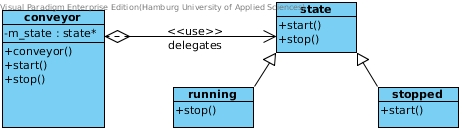
\includegraphics[scale=.6]{img/fsm_gof.jpg}
\end{frame}

%% GoF fsm States in Code I
\begin{frame}
 \frametitle{GoF States in Code I}
 \begin{itemize}
  \item Alle States erben von einer Oberstate Klasse
  \item Der Oberstate implementiert alle funktionen aller States als virtuelle Funktion
  \item Der jeweilige Status implementiert nur seine eigenen Funktionen
 \end{itemize}
\end{frame}

%% GoF fsm States in Code II (Header)
\begin{frame}[fragile]
 \frametitle{GoF States in Code II (Header)}
 \begin{lstlisting}
  struct state {
    virtual ~state() { }
    virtual void start() { }
    virtual void stop() { }
  };

  struct running : public state {
    void stop();
  };

  struct stopped : public state {
    void start();
  };
 \end{lstlisting}
\end{frame}

%% GoF fsm States in Code III (Implementierung/CPP)
\begin{frame}[fragile]
 \frametitle{GoF States in Code III}
 \begin{lstlisting}
  // transition running -> stopped
  void running::stop() {
    new (this) stopped;
    cout << "stop() / stop" << endl;
  }

  // transition stopped -> running
  void stopped::start() {
    new (this) running;
    cout << "start() / run" << endl;
  }
 \end{lstlisting}
\end{frame}

%% Placement new operator
%\begin{frame}[fragile]
% \frametitle{Placement new operator}
%\end{frame}

%% GoF fsm Kontext Klasse
\begin{frame}
 \frametitle{GoF Konext Klasse}
 \begin{itemize}
  \item Sicht von au{\ss}en auf die FSM
  \item Dient als Delegator zu den States
  \item Bedient alle Eingangssignale durch Funktionen
 \end{itemize}
\end{frame}

%% GoF fsm Konext Klasse
\begin{frame}[fragile]
 \frametitle{GoF Kontext Klasse in Code}
 Header:
 \begin{lstlisting}
  struct conveyor {
    conveyor() : m_state(new stopped) { }
    ~conveyor() { delete m_state; }
    void start();
    void stop();
   private:
    state* m_state;
  };
 \end{lstlisting}
 CPP:
 \begin{lstlisting}
  void conveyor::start() {
    m_state->start();
  }
  void conveyor::stop() {
    m_state->stop();
  }
 \end{lstlisting}
\end{frame}


%% Externe Statevariablen
\begin{frame}
 \frametitle{Externe Statevariablen}
\end{frame}

%% Entry und Exit Code
\begin{frame}
 \frametitle{Entry und Exit Code}
\end{frame}

%% History
\begin{frame}
 \frametitle{History}
\end{frame}

%% Conditions/Guards/Choice Points
\begin{frame}
 \frametitle{Conditions/Guards/Choice Points}
\end{frame}

%% Timer
\begin{frame}
 \frametitle{Timer}
\end{frame}

\end{document}